%!TEX root = ../thesis.tex

\ifpdf
    \graphicspath{{Chapter3/mt/Figs/Raster/}{Chapter3/mt/Figs/PDF/}{Chapter3/mt/Figs/}}
\else
    \graphicspath{{Chapter3/mt/Figs/Vector/}{Chapter3/mt/Figs/}}
\fi

\begin{figure}[htbp!]
\centering
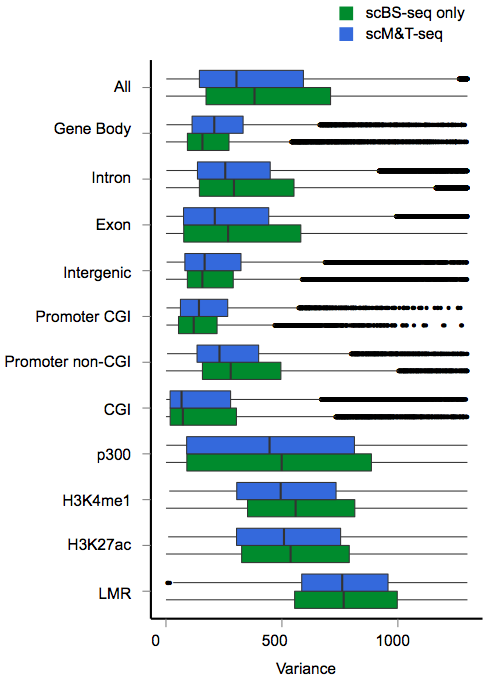
\includegraphics[width=0.6\textwidth]{var}
\caption[Comparision of epigenetic heterogeneity in cells profiled using scM\&T-seq and scBS-seq.]{Comparison of epigenetic heterogeneity in different genomic contexts, considering 61 serum ESCs obtained using scM\&T-seq and 20 serum ESCs sequenced using stand-alone scBS-seq.}
\label{fig:mt_var}
\end{figure}

\begin{figure}[htbp!]
\centering
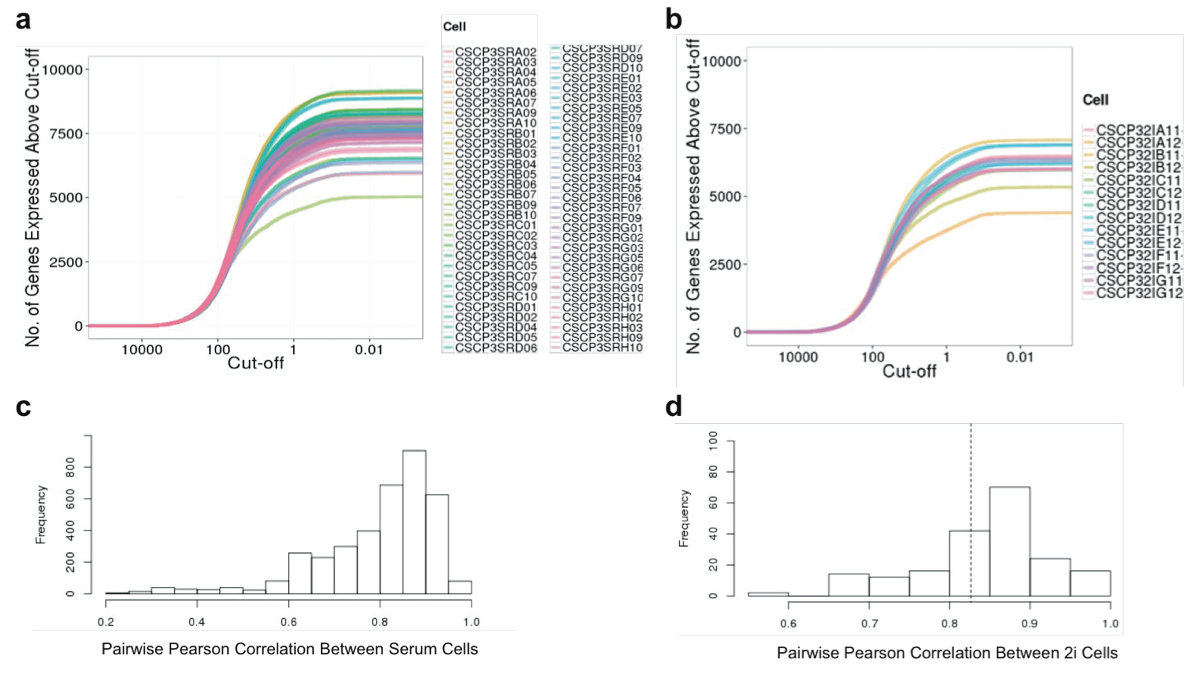
\includegraphics[width=1.0\textwidth]{qc_rna}
\caption[Quality metrics of scRNA-seq data obtained from mouse ESCs profiled using scM\&T-seq.]{Quality metrics of scRNA-seq data obtained from mouse ESCs profiled using scM\&T-seq. (a,b) Number of genes detected on (Y-axis) as a function of the expression cut off (x-axis). In each cell, between 4,000 and 8,000 genes were expressed (TPM>1) (the dashed line drawn at X=1). High quality cells generally have about 5,000 genes detectable at the cut-off of TPM>1, indicating a high level of quality among the 61 serum ESCs (or the 14 2i ESCs). (c,d) Distribution of Pearson correlation coefficient calculated pairwise on the 61 serum ESCs (or the 14 2i ESCs). The observed correlation coefficient tended to be between 0.7-0.99, indicating a high degree of technical consistency in the measured transcriptome of the cells considered, and attesting high quality of scRNA-seq data.}
\label{fig:mt_qc_rna}
\end{figure}

\begin{figure}[htbp!]
\centering
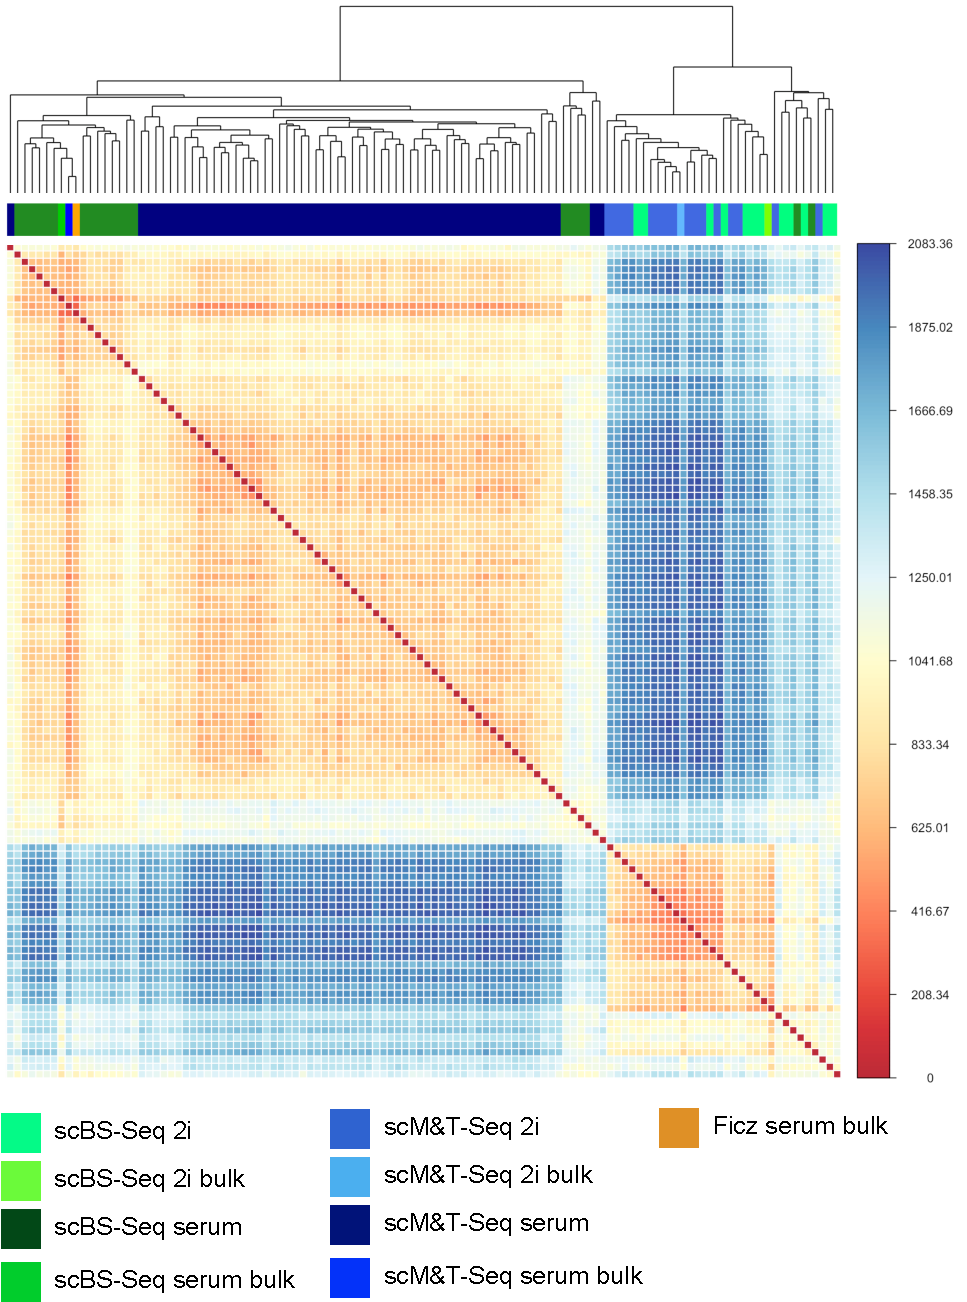
\includegraphics[width=0.8\textwidth]{clust}
\caption[Hierarchical clustering of DNA-methylation profiles generated by scM\&T-seq and scBS-seq.]{Shown s a joint hierarchical clustering from 61 serum and 16 2i cells profiled using scM\&T-seq, as well as 20 serum and 12 2i ESCs profiled by scBS-seq (Smallwood et al. 2014), as well as corresponding synthetic bulk samples and an independent bulk BS-seq sample from serum ESCs (Ficz et al. 2013). The clustering analysis was performed on gene body methylation of the 500 genes with the largest epigenome heterogeneity.}
\label{fig:mt_clust}
\end{figure}

\begin{figure}[htbp!]
\centering
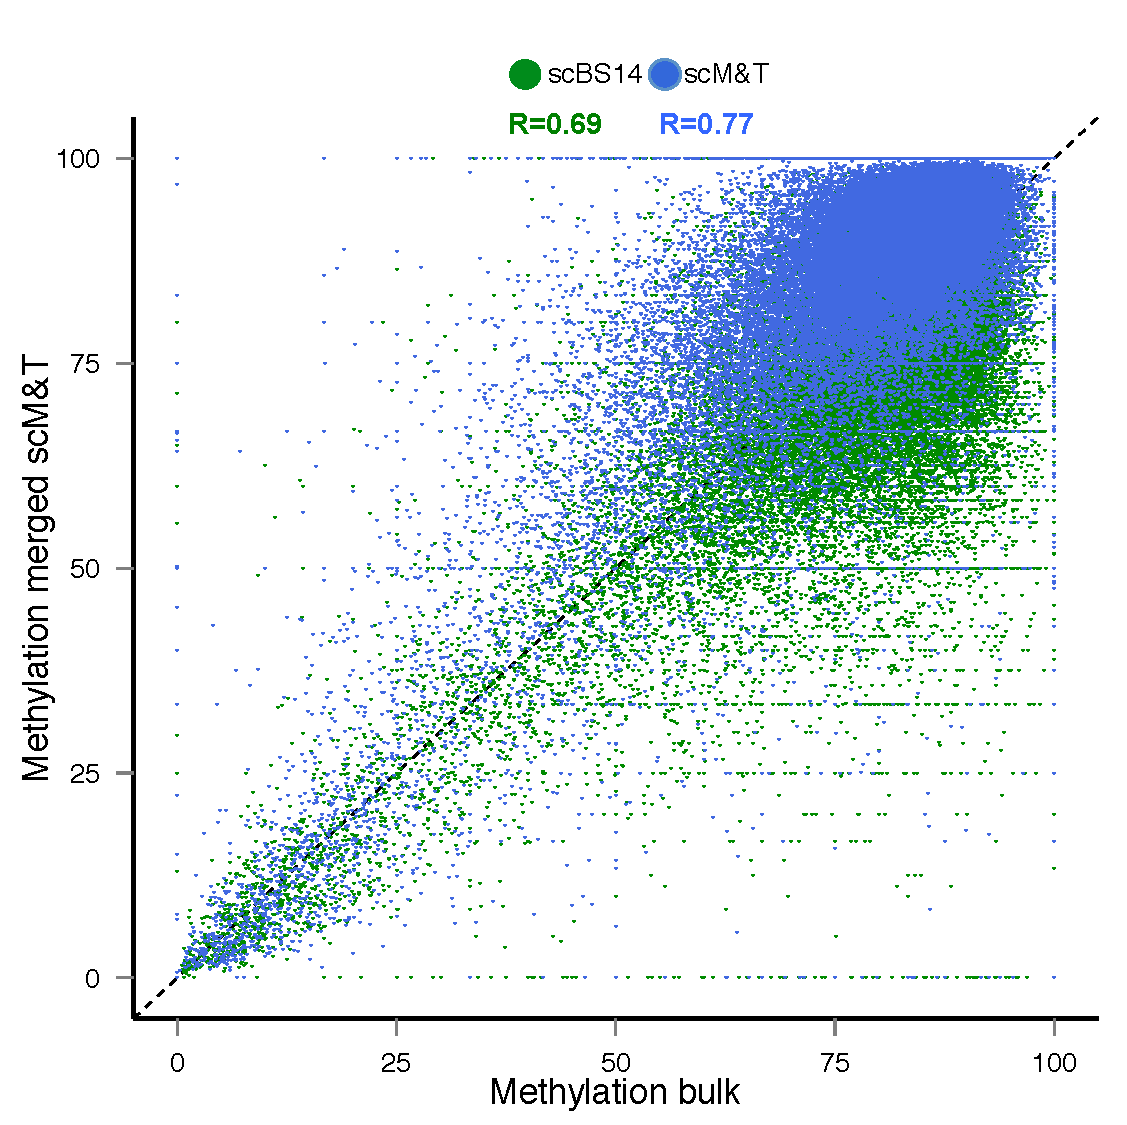
\includegraphics[width=0.7\textwidth]{bulk}
\caption[Correlation between single-cell methylomes and the methylome of a bulk cell population.]{Shown is a scatter plot, relating bulk gene-body methylation (Ficz et al. 2013) on the x-axis, versus synthetic bulk estimates of gene- body methylation derived using either scBS-seq (Smallwood et al. 2014, green) or scM\&T-seq (blue) on the y-axis. Synthetic bulk methylation profiles are derived form averages of the single-cell methylation profiles. The true bulk methylation profile is concordant with both single-cell profiles, where the scM\&T-seq bulk estimates correlate slightly better (R=0.77) than the scBS-seq bulk (R=0.69).}
\label{fig:mt_bulk}
\end{figure}

\begin{figure}[htbp!]
\centering
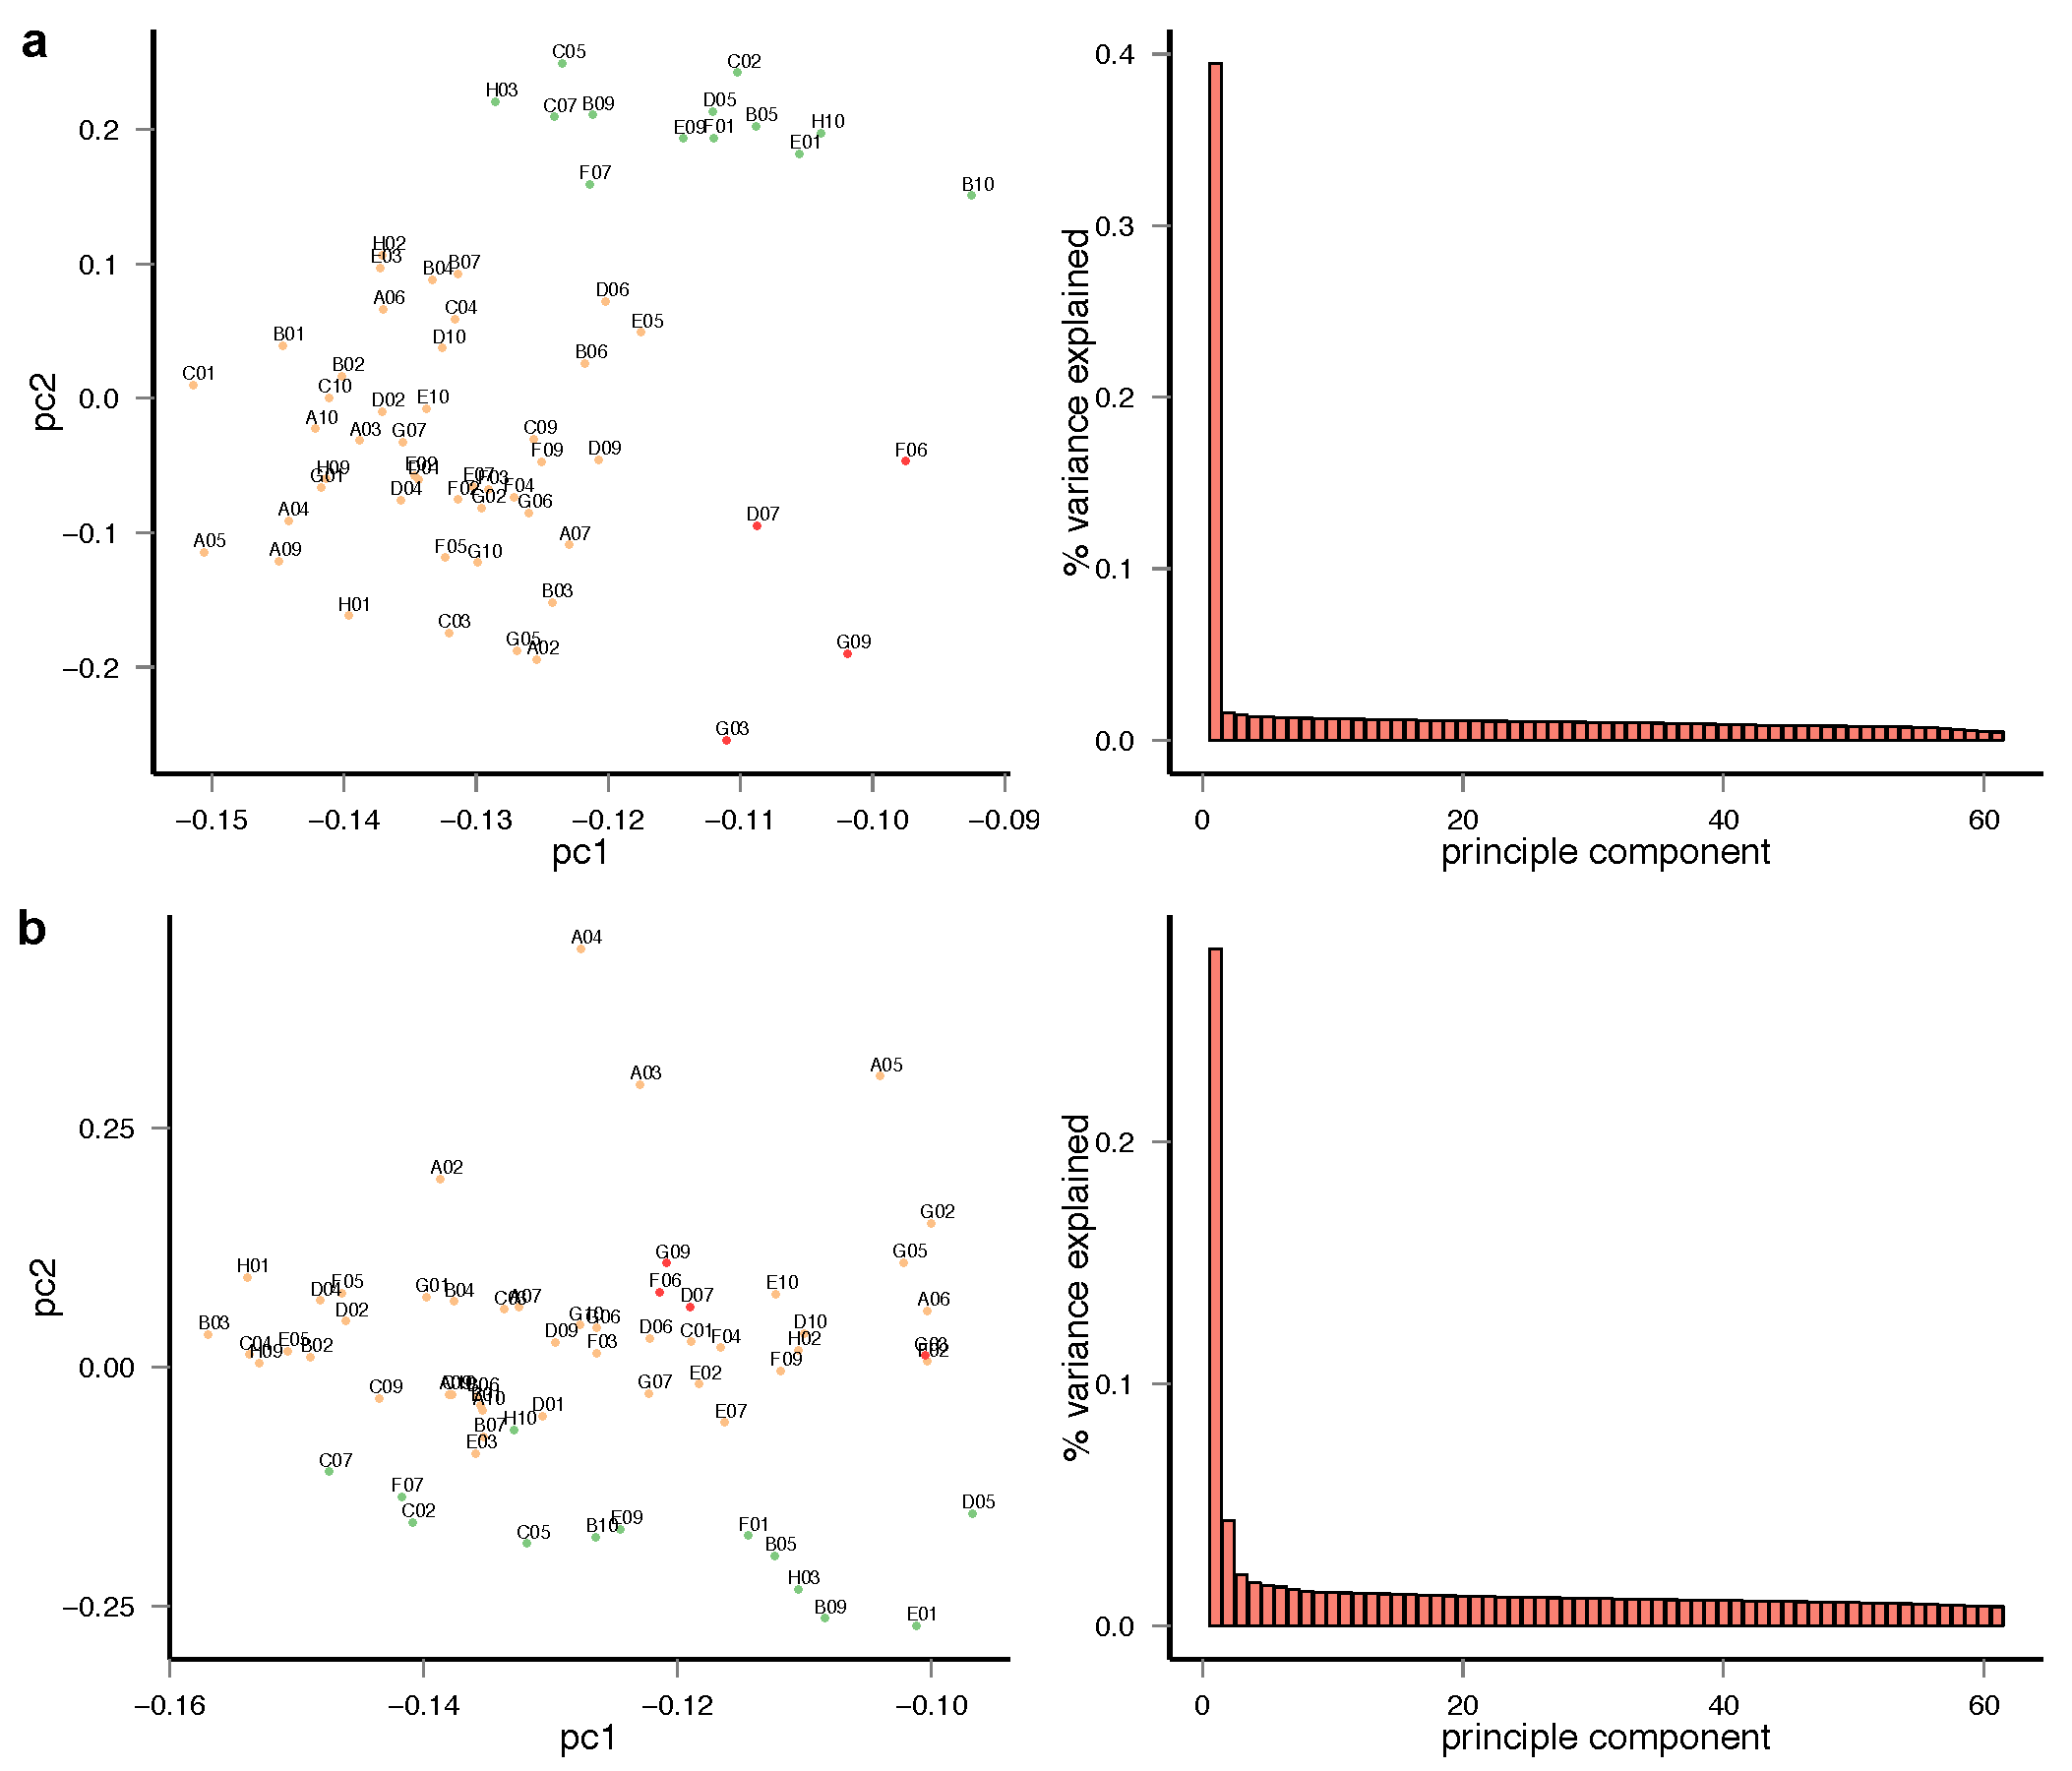
\includegraphics[width=1.0\textwidth]{cca}
\caption[Principal-component analysis of gene-body methylation and gene expression in serum-grown ESCs.]{Shown are projections onto first two principle components (left) alongside with percentage of variance explained by individual components (right) for both gene expression levels (a) and gene body methylation (b). Cells are color-coded based on clustering obtained using gene expression values, showing that that the methylation principal components partially recapitulate the structure in the expression data.}
\label{fig:mt_cca}
\end{figure}

\begin{figure}[htbp!]
\centering
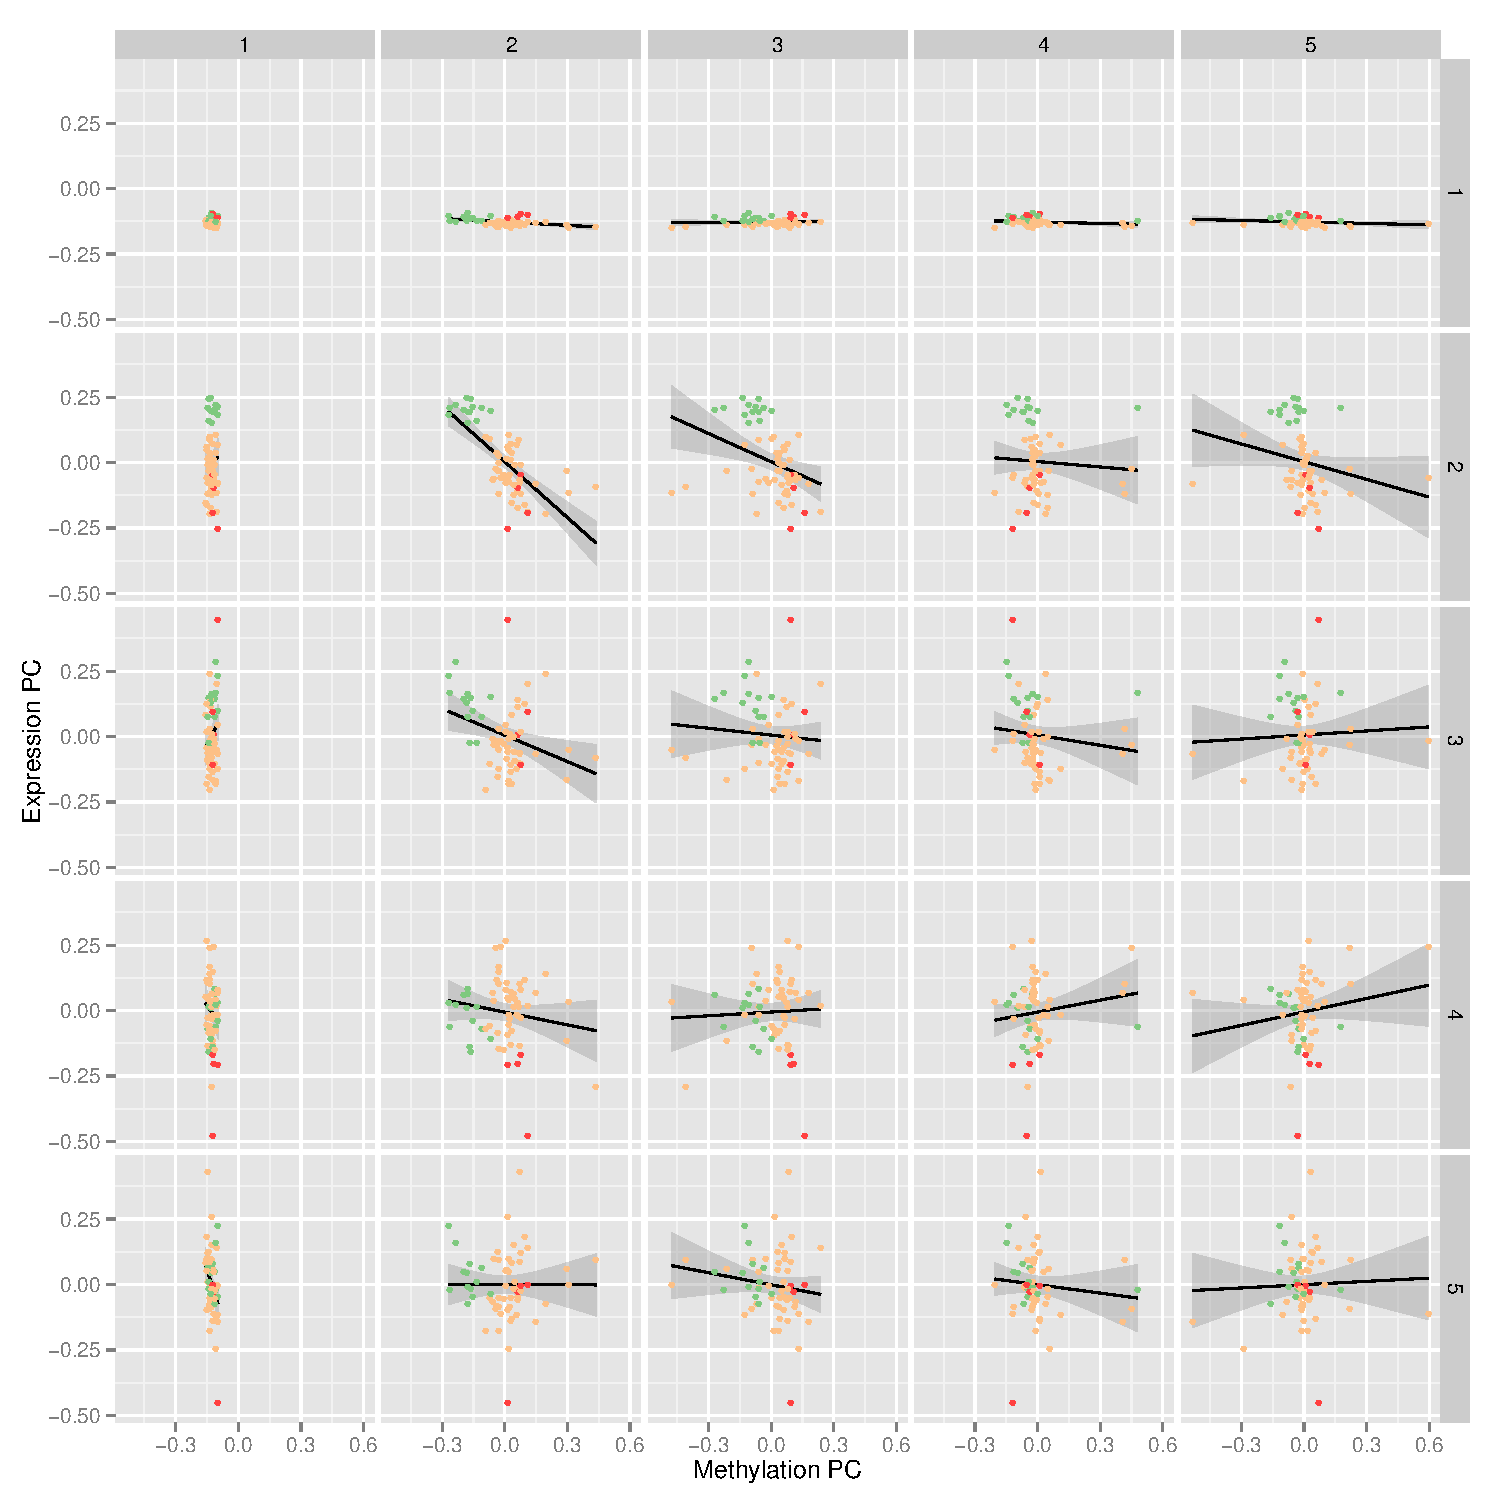
\includegraphics[width=1.0\textwidth]{cca_cor}
\caption[Scatter-plot matrix of principal components from methylation and gene expression profiles.]{Shown are scatter plots between individual principal components of gene expression levels (y-axis) and corresponding gene body methylation (x-axis), using 61 serum cells profiled using scM\&T-seq. There is a strong correlation between the second principal component of DNA methylation and the corresponding component from gene expression, suggesting shared axes of variation between transcriptome and methylome profiles.}
\label{fig:mt_cca_cor}
\end{figure}

\begin{figure}[htbp!]
\centering
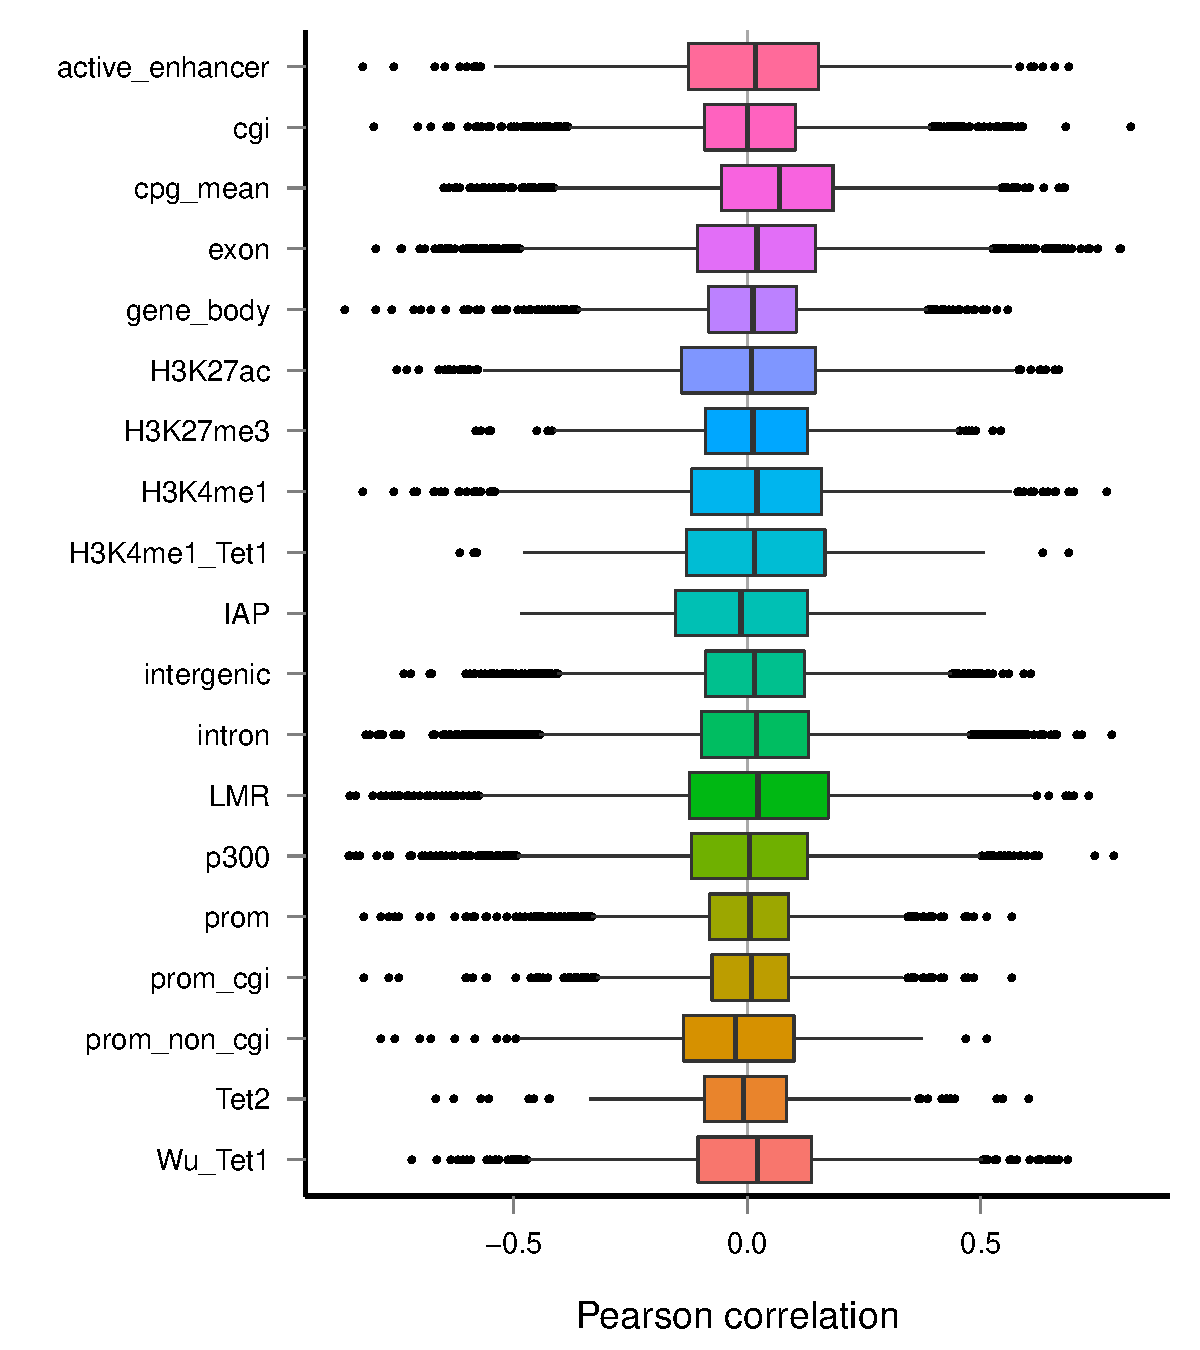
\includegraphics[width=0.8\textwidth]{gene_r}
\caption[Correlation coefficients for associations between DNA-methylation profiles in alternative genomic contexts and gene expression levels.]{Correlation coefficients for associations between DNA-methylation profiles in alternative genomic contexts and gene expression levels. Shown are boxplots of the correlation coefficient (Pearson's r) between DNA methylation in different genomic contexts and corresponding gene expression levels.}
\label{fig:mt_gene_r}
\end{figure}

\begin{figure}[htbp!]
\centering
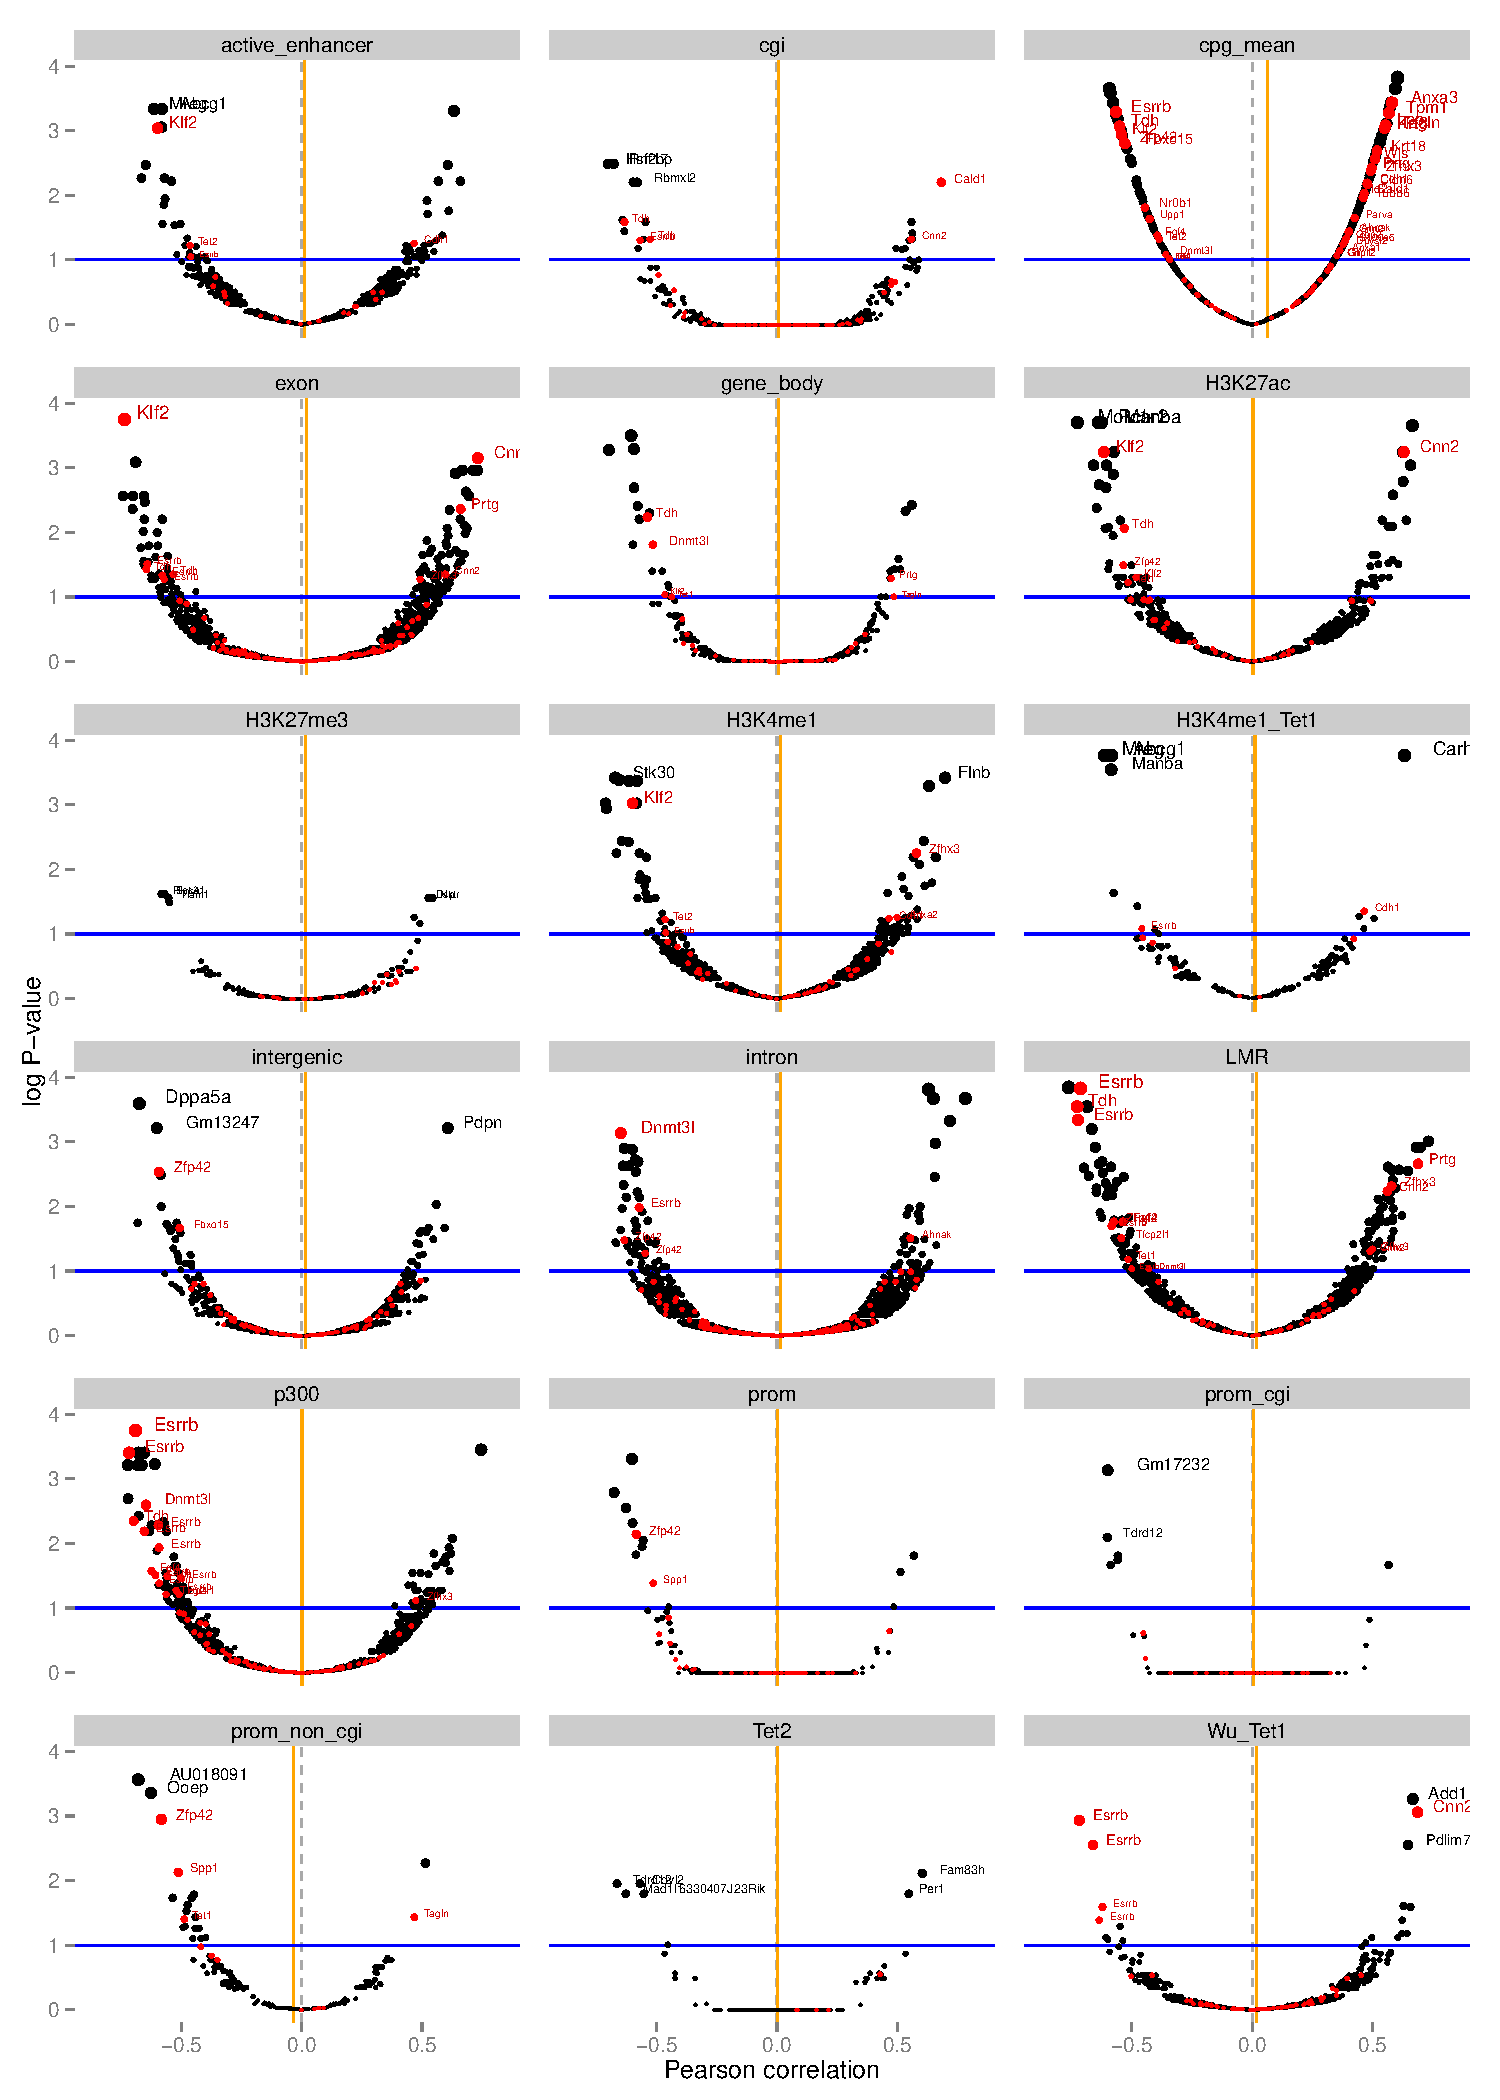
\includegraphics[width=0.9\textwidth]{gene_volcano_all}
\caption[Volcano plots for associations tests between DNA methylation profiles in alternative genomic context and gene expression levels.]{Volcano plots for associations tests between DNA methylation profiles in alternative genomic context and gene expression levels. For each context, shown is the correlation coefficient (Pearson's r, x-axis) versus the adjusted p-value (Benjamini Hochberg adjustment; y-axis). The blue horizontal line corresponds to the $\FDR=0.1$ significance level. Each dot corresponds to a gene and the size for the adjusted p-value of the association test. Genes colored in red correspond to known pluripotency genes. The vertical orange line denotes the average correlation coefficient across all genes for a given annotation.}
\label{fig:mt_gene_volcano_all}
\end{figure}

\begin{figure}[htbp!]
\centering
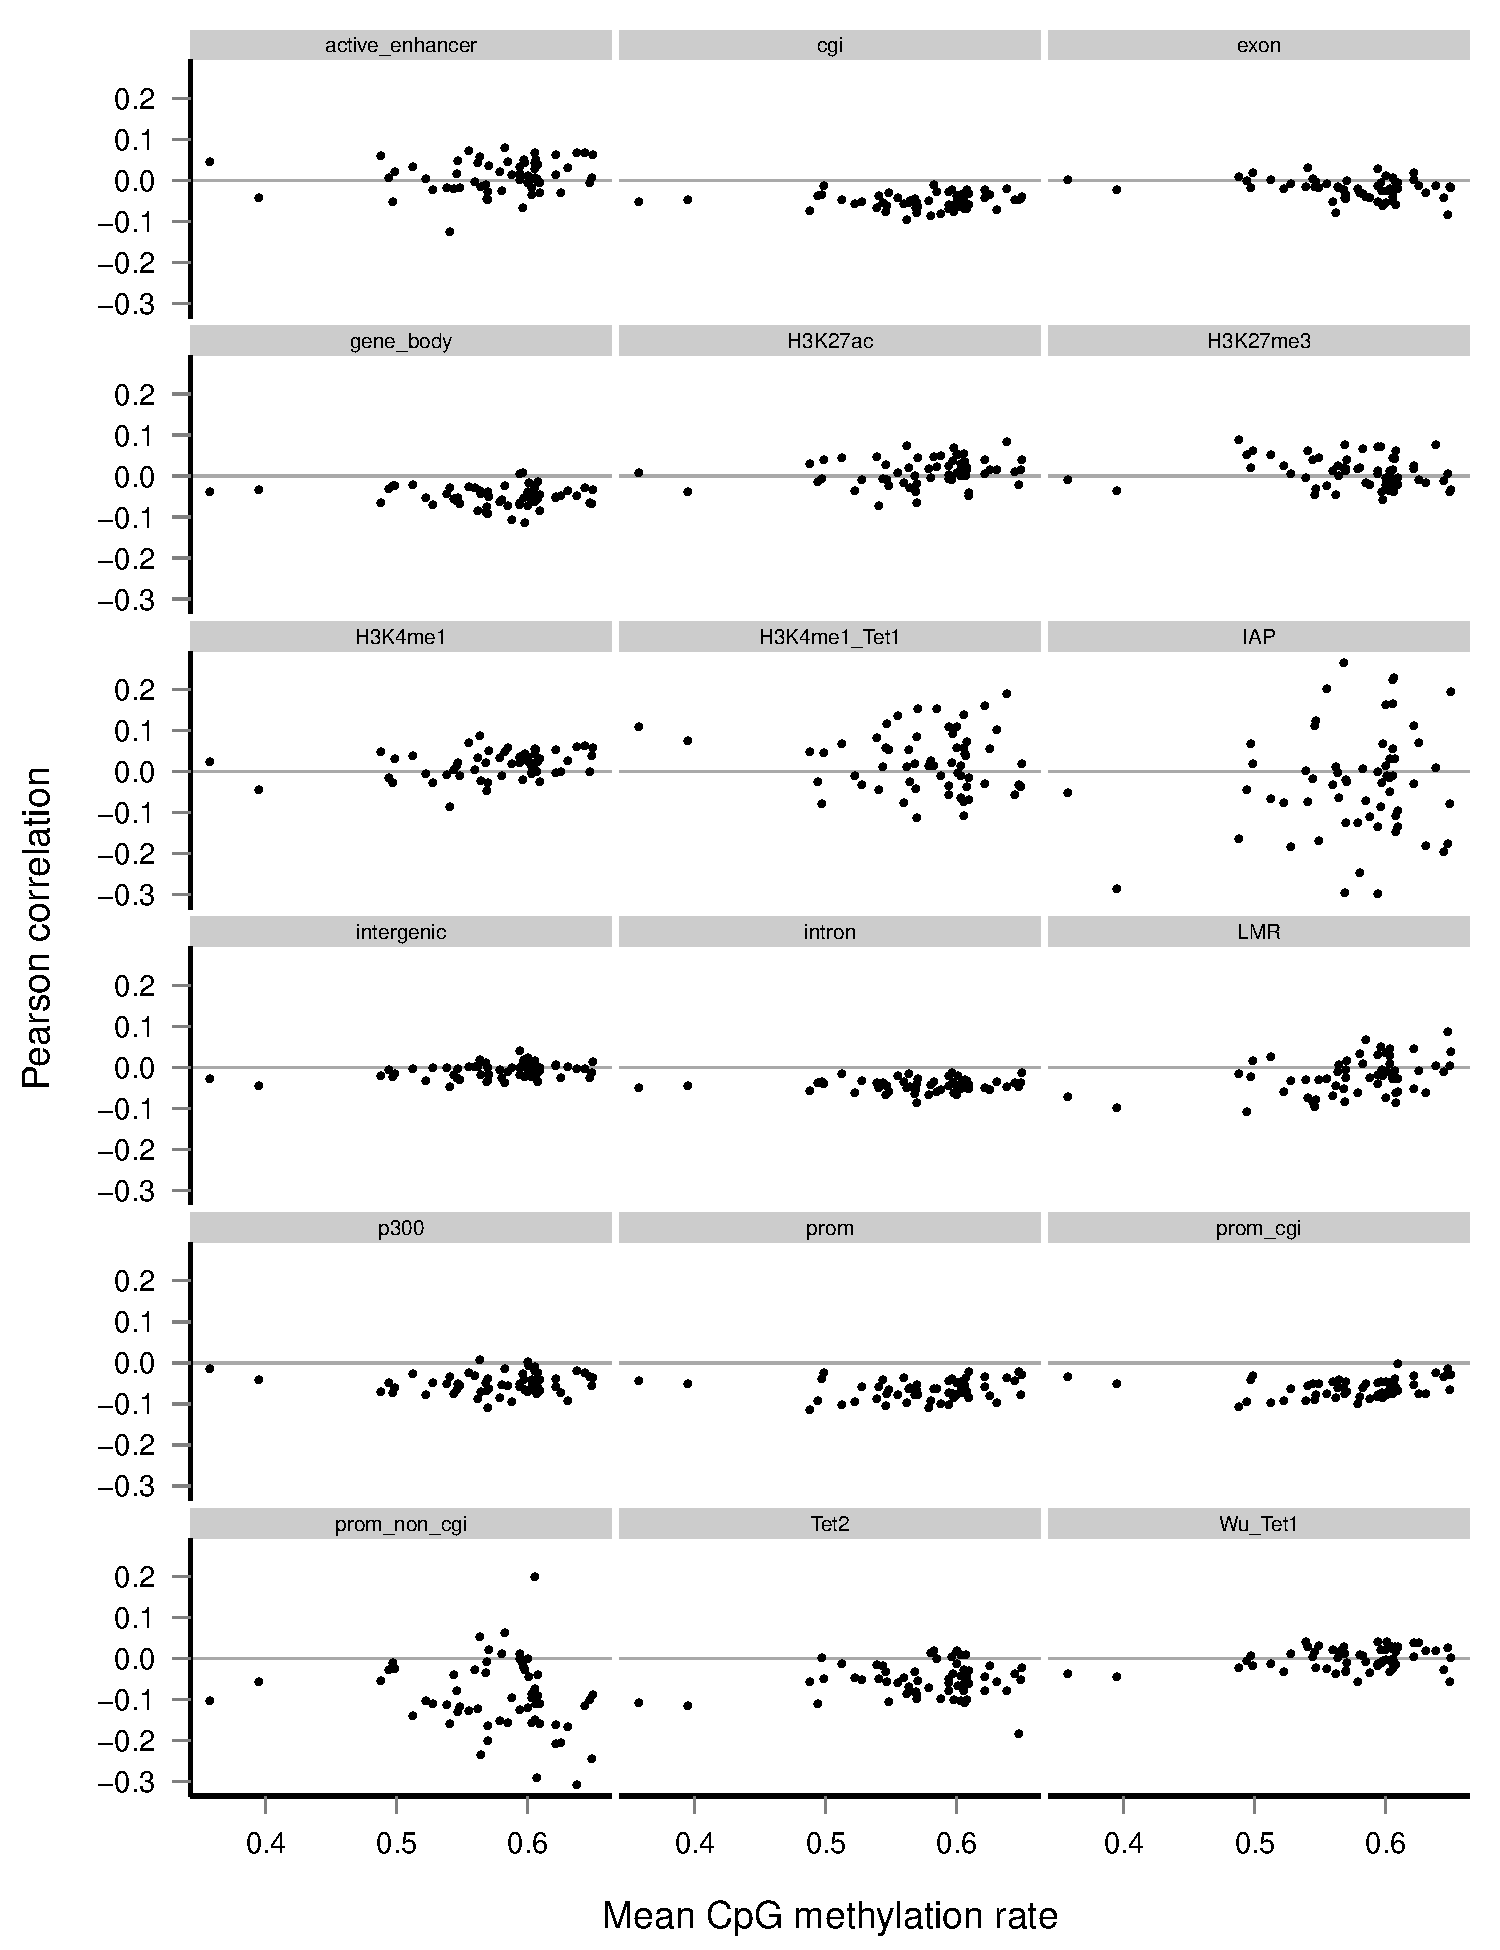
\includegraphics[width=1.0\textwidth]{cell_r_mean}
\caption{Comparison of results of cell-specific correlation analysis with mean CpG methylation rate.}
\label{fig:mt_cell_r_mean}
\end{figure}

\begin{figure}[htbp!]
\centering
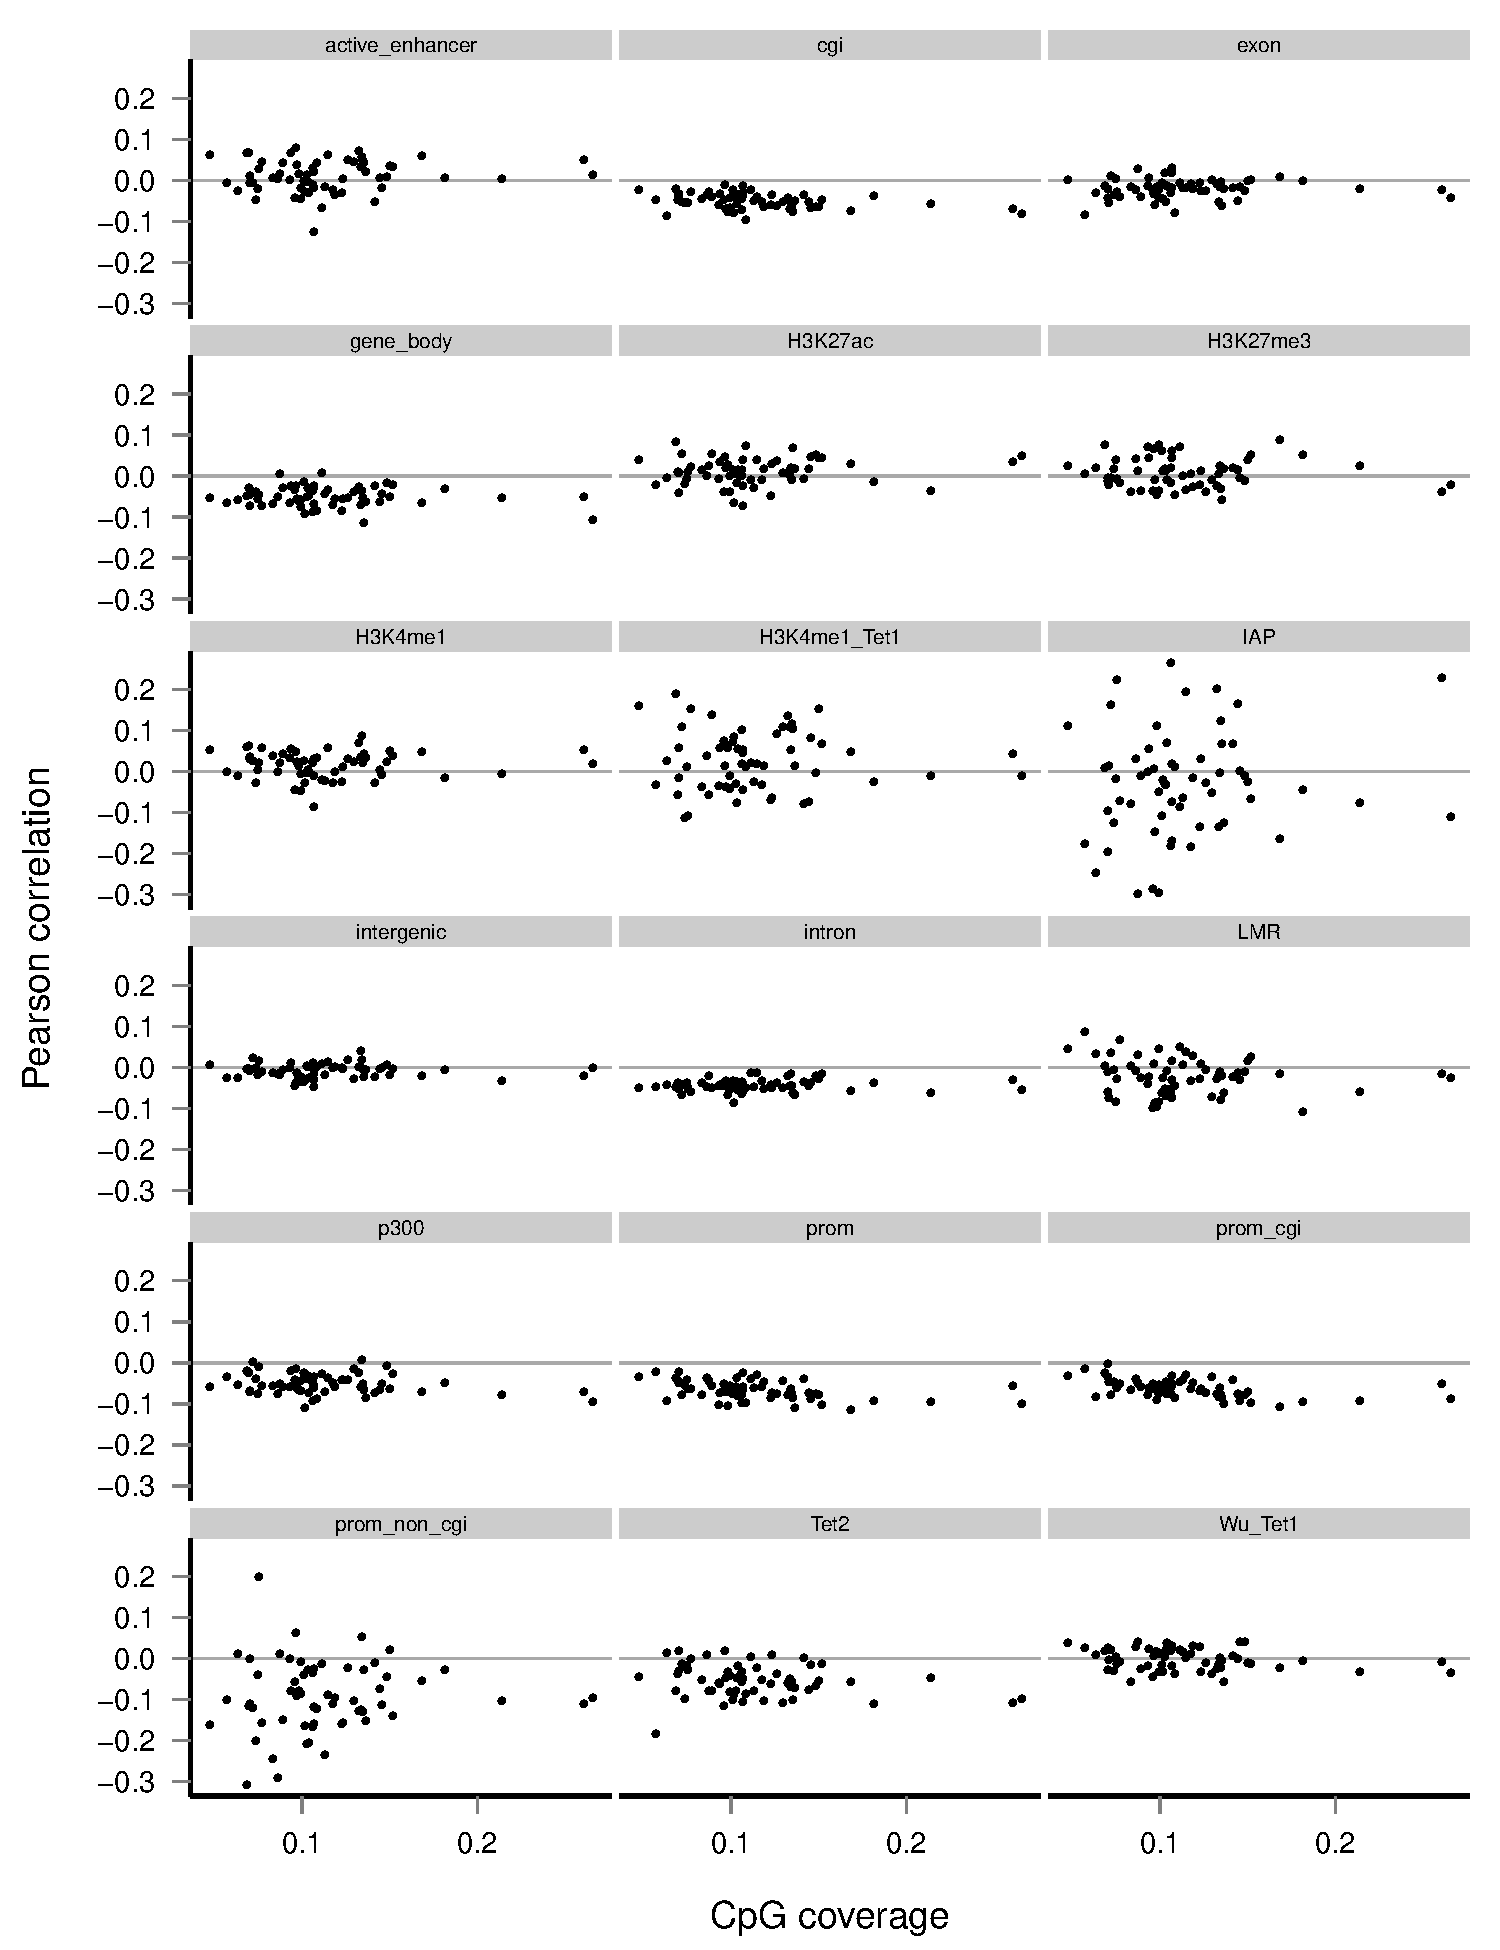
\includegraphics[width=1.0\textwidth]{cell_r_cov}
\caption{Comparison of results of cell-specific correlation analysis with CpG coverage.}
\label{fig:mt_cell_r_cov}
\end{figure}
